\chapter{Regularização}

As equações \ref{eq:sistema_normal} do problema inverso linear e
\ref{eq:sistema_normal_nlin} do problema inverso não-linear são
{\it equações normais}.
Estas equações são sistemas lineares cuja matriz é quadrada.
Para que a solução de uma equação normal seja única, é necessário que esta
matriz tenha {\it posto completo}.
Uma condição para que uma matriz tenha posto completo é que todas as suas colunas
(ou linhas) sejam {\it linearmente independentes}.
Esta condição é equivalente a dizer que a matriz possua determinante diferente de
zero.
\\
\indent Em problemas geofísicos, é comum que a matriz do sistema normal possua
determinante próximo de zero. Ou seja, para fins práticos pode-se considerar que
a matriz {\it não} tenha posto completo.
Isto faz com que o problema inverso geofísico seja um problema {\it mal posto}.

\begin{quote}
{\tt Um problema {\bf mal-posto} apresenta, principalmente, {\it instabilidade}
e {\it falta de unicidade} da solução.}
\end{quote}

\indent A instabilidade é definida como

\begin{quote}
{\tt A {\bf instabilidade} é a alta variabilidade dos parâmetros perante
peque\-nas variações nos dados.}
\end{quote}

\noindent Por exemplo, seja um conjunto de dados preditos A e outro conjunto de
dados preditos ligeiramente diferentes B.
Se o problema inverso apresenta instabilidade, os pa\-râ\-me\-tros que produzem os
dados preditos A são consideravelmente diferentes daqueles que produzem os dados
preditos B.
\\
\indent A falta de unicidade é definida como

\begin{quote}
{\tt A {\bf falta de unicidade} é a existência de vários conjuntos de parâme\-tros
que produzem os mesmos dados preditos.}
\end{quote}

\noindent Em outras palavras, os dados observados podem ser explicados por vários
conjuntos de parâmetros diferentes. Em termos práticos, existem vários vetores
de parâmetros diferentes que minimizam a função do ajuste
(equação \ref{eq:ajuste}).
\\
\indent Os problemas inversos encontrados na geofísica são, em geral, mal-postos.
Os principais motivos para isto são: a presença de ruído nos dados observados; e,
principalmente, a própria natureza do problema inverso.
Ou seja, mesmo se fôssemos capazes de obter dados completamente isentos de ruído, ainda
teríamos diversas combinações de parâmetros capazes de explicar os dados
observados (i.e., falta de unicidade).
Por este motivo, quando nos deparamos com problemas inversos na geofísica,
é essencial a utilização de {\it regularização}.
\\
\indent A {\it regularização} é um procedimento matemático que contorna os
problemas de ins\-tabilidade e falta de unicidade em problemas inversos mal-postos.
Esse procedimento equivale a impor restrições aos parâmetros a serem estimados.
Desta forma, em um {\it problema inverso regularizado} buscamos estimar um
conjunto de parâmetros que ajustam os dados observados e satisfaçam
determinadas restrições.
Estas restrições introduzem informações {\it a priori} no problema inverso.
As informações podem ser de natureza geológica ou meramente matemática.
Em geral, a introdução de informações a priori é feita por meio de {\it funções
regularizadoras}.
Estas funções são funções escalares que dependem dos parâmetros.
Para vincular uma função regularizadora ao ajuste dos dados, formamos a
{\it função objetivo}

\begin{equation}
\Omega(\vect{p}) = \phi(\vect{p}) + \mu\theta(\vect{p}) \thinspace ,
\label{eq:objetivo}
\end{equation}

\noindent em que $\phi(\vect{p})$ é a função do ajuste (equação \ref{eq:ajuste}),
$\theta(\vect{p})$ é uma função regularizadora e $\mu$ é um escalar positivo
denominado {\it parâmetro de regularização}.
Desta forma, o {\it problema inverso regularizado} é definido como estimar um
vetor de parâmetros $\opt{p}$ que {\it minimiza a função objetivo}.
\\
\indent Neste ponto é importante ressaltar que

\begin{quote}
{\tt O {\bf parâmetro de regularização} $\mu$ controla a importância relativa
en\-tre o ajuste aos dados observados e a concordância com a infor\-ma\-ção
a priori.}
\end{quote}

\noindent O valor de $\mu$ é definido pelo usuário da inversão e por isso é
importante compreender sua influência no resultado obtido (parâmetros estimados).
Valores altos de $\mu$ tornam o problema inverso bem posto e fazem com que os
parâmetros estimados satisfaçam quase completamente as informações a priori.
Porém, isto geralmente faz com que haja um desajuste entre os dados observados e
preditos.
Por outro lado, valores baixos de $\mu$ fazem com que os parâmetros estimados
ajustem os dados observados. No entanto, a estimativa poderá ser não-única e/ou
instável, dependendo de quanto o problema inverso for mal-posto.
Idealmente, deve-se encontrar um valor de $\mu$ que proporcione um bom ajuste e
satisfaça as informações a priori o suficiente para estabilizar a solução.
Procedimentos práticos para determinação do valor de $\mu$ serão discutidos no
Capítulo \ref{chap:proc_praticos}.
\\
\indent No problema inverso regularizado, a linearidade não depende apenas da
função $f_i(\vect{p})$ (equação \ref{eq:fi}) que relaciona os parâmetros aos
dados preditos, mas também da função regularizadora.
Nesse caso, para que o problema inverso seja linear, é necessário que tanto
$f_i(\vect{p})$ como o {\it gradiente da função regularizadora} sejam
combinações lineares dos parâmetros.
Se ao menos uma destas funções for não-linear, o problema inverso deverá ser
resolvido como um problema inverso não-linear.
\\
\indent Como foi observado anteriormente (Seção \ref{sec:nao-linear}), o
problema inverso linear é um caso particular do problema inverso não-linear.
Por esta razão, a formulação geral para o problema inverso regularizado
será feita seguindo os procedimentos adotados para o problema inverso não-linear.
Assim sendo, iniciaremos expandindo a função objetivo (equação
\ref{eq:objetivo}) em série de Taylor até segunda ordem

\begin{equation}
\Omega(\vect{p}_0 + \Delta\vect{p}) \approx \Omega(\vect{p}_0) +
    \vect{\nabla}\Omega(\vect{p}_0)^T\Delta\vect{p} +
    \frac{1}{2}\Delta\vect{p}^T\mat{\nabla}\Omega(\vect{p}_0)\Delta\vect{p}
    \thinspace ,
\label{eq:objetivo_taylor}
\end{equation}

\noindent sendo o vetor gradiente $\vect{\nabla}\Omega(\vect{p}_0)$ e a matriz
Hessiana $\mat{\nabla}\Omega(\vect{p}_0)$ de $\Omega(\vect{p})$ dados por

\begin{equation}
\vect{\nabla}\Omega(\vect{p}_0) = \vect{\nabla}\phi(\vect{p}_0) +
    \mu\vect{\nabla}\theta(\vect{p}_0) \thinspace
\label{eq:grad_objetivo}
\end{equation}

\noindent e

\begin{equation}
\mat{\nabla}\Omega(\vect{p}_0) = \mat{\nabla}\phi(\vect{p}_0) +
    \mu\mat{\nabla}\theta(\vect{p}_0) \thinspace ,
\label{eq:hessian_objetivo}
\end{equation}

\noindent em que $\mu$ é o parâmetro de regularização,
$\vect{\nabla}\phi(\vect{p}_0)$ e $\mat{\nabla}\phi(\vect{p}_0)$
são o gradiente e a Hessiana da função do ajuste (equações \ref{eq:gradphi} e
\ref{eq:hessian_approx}) e
$\vect{\nabla}\theta(\vect{p}_0)$ e $\mat{\nabla}\theta(\vect{p}_0)$ são o
gradiente e a Hessiana da função regularizadora, todos avaliados em $\vect{p}_0$.
\\
\indent Seguindo a dedução feita para o problema inverso não-linear (Seção
\ref{sec:nao-linear}), a correção $\Delta\vect{p}$ em uma determinada iteração
do método Gauss-Newton é

\begin{equation}
\mat{\nabla}\Omega(\vect{p}_0)\Delta\vect{p} = -\vect{\nabla}\Omega(\vect{p}_0)
    \thinspace .
\label{eq:sistema_normal_objetivo}
\end{equation}

\noindent Substituindo o gradiente e a Hessiana da função do ajuste (equações
\ref{eq:gradphi} e \ref{eq:hessian_approx}) obtemos

\begin{equation}
\left[\mat{G}(\vect{p}_0)^T\mat{G}(\vect{p}_0) +
      \frac{1}{2}\mu\mat{\nabla}\theta(\vect{p}_0)\right]\Delta\vect{p} =
\mat{G}(\vect{p}_0)^T \left[\vect{d}^{\thinspace o} - \vect{f}(\vect{p}_0)\right] -
\frac{1}{2}\mu\vect{\nabla}\theta(\vect{p}_0)
    \thinspace .
\label{eq:sistema_normal_regul}
\end{equation}

\indent A equação \ref{eq:sistema_normal_regul} é a equação normal para o
{\it problema inverso regularizado}.\footnote{Tente obter a equação normal para
o caso em que $\vect{f}(\vect{p})$ é linear.}
A seguir, apresentaremos diferentes funções regularizadoras comumente encontradas
em problemas inversos na geofísica.
Também mostraremos como fica a equação \ref{eq:sistema_normal_regul} para cada
um dos casos.

\section{Norma mínima (Tikhonov de ordem 0)}

A função regularizadora mais comumente usada é a chamada {\it norma mínima}
(também conhecida como {\it ridge regression} ou {\it Tikhonov de ordem zero}).
Como seu nome sugere, esta função é utilizada para incorporar a informação de
que o vetor de parâmetros deve ter a norma quadrática ($\ell_2$ ou Euclidiana)
mínima.
Isto é, os parâmetros devem ser assumir valores mais próximos possíveis a zero.
De forma similar a equação \ref{eq:dotprod}, a função regularizadora de norma
mínima tem a seguinte forma

\begin{equation}
\theta^{NM}(\vect{p}) = \vect{p}^T\vect{p} \thinspace .
\label{eq:norma_minima}
\end{equation}

\indent O vetor gradiente $\vect{\nabla}\theta^{NM}(\vect{p})$ e a matriz Hessiana
$\mat{\nabla}\theta^{NM}(\vect{p})$ (ver Apêndice \ref{chap:opmat}) desta função
são, respectivamente,

\begin{equation}
\vect{\nabla}\theta^{NM}(\vect{p}) = 2\mat{I}\vect{p}
\label{eq:grad_norma_minima}
\end{equation}

\noindent e

\begin{equation}
\mat{\nabla}\theta^{NM}(\vect{p}) = 2\mat{I} \thinspace ,
\label{eq:hessian_norma_minima}
\end{equation}

\noindent em que $\mat{I}$ é a matriz identidade de dimensão $M \times M$,
lembrando que $M$ é o número de parâmetros.
Note que o gradiente da função regularizadora de norma mínima é uma
{\it combinação linear dos parâmetros}.
\\
\indent Para o caso em que a função $f_i(\vect{p})$ que relaciona
os dados preditos aos parâmetros também é {\it linear} (equação \ref{eq:comb_linear}),
a equação normal do {\it problema inverso linear regularizado},
para o caso da regularização de norma mínima\footnote{
Onde foi parar o termo $\vect{\nabla}\theta^{NM}(\vect{p}_0)$? Dica: Mostre que, se o
problema inverso é linear, a estimativa $\opt{p}$ não depende da aproximação
inicial $\vect{p}_0$.}, é

\begin{equation}
\left(\mat{G}^T\mat{G} + \mu\mat{I}\right)\opt{p} =
    \mat{G}^T\left(\vect{d}^{\thinspace o} - \vect{b} \right) ,
\label{eq:sistema_normal_norma_min_linear}
\end{equation}

\noindent em que $\mu$ é o parâmetro de regularização, $\vect{d}^{\thinspace o}$
é o vetor de dados observados, $\mat{G}$ é a matriz de sensibilidade, $\vect{b}$
é um vetor de constantes (equação \ref{eq:f_igual_Gp}) e $\opt{p}$ é a solução
de norma mínima para o problema inverso linear.
\\
\indent Já para o caso em que $f_i(\vect{p})$ é {\it não-linear}, o problema
inverso torna-se também não-linear. Assim sendo, a equação normal do
{\it problema inverso não-linear regularizado}, para o caso da regularização de
norma mínima, é

\begin{equation}
\left[\mat{G}(\vect{p}_0)^T\mat{G}(\vect{p}_0) +
      \mu\mat{I}\right]\Delta\vect{p} =
\mat{G}(\vect{p}_0)^T \left[\vect{d}^{\thinspace o} - \vect{f}(\vect{p}_0)\right] -
\mu\vect{p}_0
    \thinspace .
\label{eq:sistema_normal_norma_min_naolinear}
\end{equation}

\noindent em que $\vect{f}(\vect{p}_0)$ é o vetor de dados preditos avaliado em
$\vect{p}_0$ e $\Delta\vect{p}$ é a correção a ser aplicada a $\vect{p}_0$
que leva à solução de norma mínima.

\section{Suavidade (Tikhonov de ordem 1)}
\label{sec:smoothness}

Em certas situações é desejável que a distribuição dos parâmetros seja ``suave''.
Existem diversas interpretações para esta restrição, porém a mais comum é que
parâmetros espacialmente adjacentes devem ter valores mais próximos possível.
Em outras palavras, não devem haver variações abruptas entre parâmetros
espacialmente adjacentes, ou que a diferença entre estes parâmetros deve ser
mínima.
\\
\indent A função regularizadora utilizada para incorporar a informação de
suavidade tem a seguinte forma

\begin{equation}
\theta^{SV}(\vect{p}) = \vect{v}^T\vect{v} \thinspace ,
\end{equation}

\noindent em que $\vect{v}$ é um vetor com as diferêncas entre os parâmetros
espacialmente adjacentes. O vetor $\vect{v}$ é uma aproximação de diferenças
finitas para a derivada espacial dos parâmetros e pode ser escrito como

\begin{equation}
\vect{v} = \mat{R}\thinspace\vect{p} \thinspace ,
\label{eq:vetor_diferencas}
\end{equation}

\noindent em que $\mat{R}$ é uma matriz de diferenças finitas.

\begin{example}
Seja o problema inverso de estimar o relevo de uma bacia
sedimentar. Uma possível parametrização seria discretizar a bacia em 7 prismas
retangulares justapostos com larguras fixas. Os parâmetros a serem estimados
seriam então as 7 espessuras dos prismas (Figura \ref{fig:basin-smoothness}).
Impor suavidade ao relevo da bacia é equivalente a minimizar as diferenças
$p_1 - p_2$, $p_2 - p_3$, $p_3 - p_4$, $p_4 - p_5$, $p_5 - p_6$ e $p_6 - p_7$.
Neste caso, o vetor $\vect{v}$ das diferenças entre os parâmetros espacialmente
adjacentes é dado por

\begin{equation}
\vect{v} =
    \begin{bmatrix}
    p_1 - p_2 \\ p_2 - p_3 \\ p_3 - p_4 \\ p_4 - p_5 \\ p_5 - p_6 \\ p_6 - p_7
    \end{bmatrix}
    =
    \underbrace{
    \begin{bmatrix}
    1 & -1 & 0 & 0 & 0 & 0 & 0\\
    0 & 1 & -1 & 0 & 0 & 0 & 0\\    
    0 & 0 & 1 & -1 & 0 & 0 & 0\\    
    0 & 0 & 0 & 1 & -1 & 0 & 0\\    
    0 & 0 & 0 & 0 & 1 & -1 & 0\\    
    0 & 0 & 0 & 0 & 0 & 1 & -1\\    
    \end{bmatrix}}_{\mat{R}}    
    \underbrace{
    \begin{bmatrix}
    p_1 \\ p_2 \\ p_3 \\ p_4 \\ p_5 \\ p_6 \\ p_7
    \end{bmatrix}}_{\vect{p}}    
     \thinspace .
\end{equation}

\begin{figure}
    \centering
    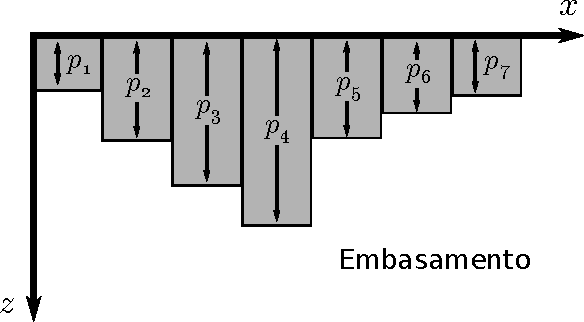
\includegraphics[scale=1]{figs/basin-smoothness}
    \caption{Exemplo de parametrização do relevo de uma bacia sedimentar.
    Neste caso, os 7 parâmetros utilizados são as espessuras de prismas
    retangulares justapostos. Impor suavidade ao relevo da bacia é equivalente
    a minimizar as diferenças $p_1 - p_2$, $p_2 - p_3$, $p_3 - p_4$, $p_4 - p_5$,
    $p_5 - p_6$ e $p_6 - p_7$.}
    \label{fig:basin-smoothness}
\end{figure}

\end{example}

\indent A {\it função regularizadora de suavidade} (também conhecida como
{\it Tikhonov de ordem um}) pode ser escrita como 

\begin{equation}
\theta^{SV}(\vect{p}) = \vect{p}^T \mat{R}^T \mat{R}\thinspace\vect{p} \thinspace .
\label{eq:suavidade}
\end{equation}

\noindent O vetor gradiente $\vect{\nabla}\theta^{SV}(\vect{p})$ e a matriz Hessiana
$\mat{\nabla}\theta^{SV}(\vect{p})$ (ver Apêndice \ref{chap:opmat}) desta função
são, respectivamente,

\begin{equation}
\vect{\nabla}\theta^{SV}(\vect{p}) = 2\mat{R}^T \mat{R}\thinspace\vect{p}
\end{equation}

\noindent e

\begin{equation}
\mat{\nabla}\theta^{SV}(\vect{p}) = 2\mat{R}^T \mat{R} \thinspace .
\end{equation}

\indent O gradiente da função regularizadora de norma mínima é uma
{\it combinação linear dos parâmetros}.
Para o caso em que a função $f_i(\vect{p})$ que relaciona
os dados preditos aos parâmetros também é {\it linear} (equação \ref{eq:comb_linear}),
a equação normal do {\it problema inverso linear regularizado},
para o caso da regularização de suavidade, é

\begin{equation}
\left(\mat{G}^T\mat{G} + \mu\mat{R}^T\mat{R}\right)\opt{p} =
    \mat{G}^T\left(\vect{d}^{\thinspace o} - \vect{b} \right) ,
\end{equation}

\noindent em que $\mu$ é o parâmetro de regularização, $\vect{d}^{\thinspace o}$
é o vetor de dados observados, $\mat{G}$ é a matriz de sensibilidade, $\vect{b}$
é um vetor de constantes (equação \ref{eq:f_igual_Gp}) e $\opt{p}$ é a solução
suave para o problema inverso linear.
\\
\indent Já para o caso em que $f_i(\vect{p})$ é {\it não-linear}, o problema
inverso torna-se também não-linear. Assim sendo, a equação normal do
{\it problema inverso não-linear regularizado}, para o caso da regularização de
suavidade, é

\begin{equation}
\left[\mat{G}(\vect{p}_0)^T\mat{G}(\vect{p}_0) +
      \mu\mat{R}^T\mat{R}\right]\Delta\vect{p} =
\mat{G}(\vect{p}_0)^T \left[\vect{d}^{\thinspace o} - \vect{f}(\vect{p}_0)\right] -
\mu\mat{R}^T\mat{R}\thinspace\vect{p}_0
    \thinspace .
\end{equation}

\noindent em que $\vect{f}(\vect{p}_0)$ é o vetor de dados preditos avaliado em
$\vect{p}_0$ e $\Delta\vect{p}$ é a correção a ser aplicada a $\vect{p}_0$.

\section{Igualdade}

meh
bla

\section{Variação total}

Ao contrário do que vimos na Seção \ref{sec:smoothness}, há situações em que é
desejável que hajam algumas {\it discontinuidades} entre parâmetros espacialmente
adjacentes. Nestes casos, podemos utilizar a função regularizadora de
{\it variação total}

\begin{equation}
\theta^{VT}(\vect{p}) = \sum\limits_{k=1}^L |v_k| \thinspace ,
\end{equation}

\noindent em que $v_k$, $k=1,2,\dotsc,L$, é o $k$-ésimo elemento do vetor de
diferenças $\vect{v}$ (equação \ref{eq:vetor_diferencas}).
Como esta função não é diferenciável para valores de $v_k = 0$, podemos
aproximá-la por

\begin{equation}
\theta^{VT}(\vect{p}) \approx \theta^{VT}_\beta(\vect{p}) =
    \sum\limits_{k=1}^L \sqrt{v_k^2 + \beta} \thinspace ,
\end{equation}

\noindent sendo $\beta$ um escalar positivo pequeno.
\\
\indent O vetor gradiente $\vect{\nabla}\theta^{VT}_\beta(\vect{p})$ e a matriz
Hessiana $\mat{\nabla}\theta^{VT}_\beta(\vect{p})$ desta função
são, respectivamente, \citep{martins_etal2011}

\begin{equation}
\vect{\nabla}\theta^{VT}_\beta(\vect{p}) = \mat{R}^T \vect{q}(\vect{p})
\label{eq:grad_tv}
\end{equation}

\noindent e

\begin{equation}
\mat{\nabla}\theta^{VT}_\beta(\vect{p}) = \mat{R}^T \mat{Q}(\vect{p})\mat{R}
\thinspace ,
\label{eq:hessian_tv}
\end{equation}

\noindent
sendo $\mat{R}$ uma matriz de diferenças finitas
(equação \ref{eq:vetor_diferencas}).
O vetor $\vect{q}(\vect{p})$ e a matriz $\mat{Q}(\vect{p})$ são, respectivamente,

\begin{equation}
\vect{q}(\vect{p}) =
    \begin{bmatrix}
    \dfrac{v_1}{\sqrt{v_1^2 + \beta}} \vspace{0.3cm}\\
    \dfrac{v_2}{\sqrt{v_2^2 + \beta}} \\
    \vdots \\ \dfrac{v_L}{\sqrt{v_L^2 + \beta}}
    \end{bmatrix} \thinspace
\end{equation}

\noindent e

\begin{equation}
\mat{Q}(\vect{p}) =
    \begin{bmatrix}
    \dfrac{\beta}{(v_1^2 + \beta)^{\frac{3}{2}}} & 0 & \ldots & 0 \vspace{0.3cm}\\
    0 & \dfrac{\beta}{(v_2^2 + \beta)^{\frac{3}{2}}} & \ldots & 0 \\
    \vdots & \vdots & \ddots & \vdots \\
    0 & 0 & \ldots & \dfrac{\beta}{(v_L^2 + \beta)^{\frac{3}{2}}}
    \end{bmatrix} \thinspace .
\end{equation}

\indent Como o gradiente e a Hessiana da função regularizadora de variação
total (equações \ref{eq:grad_tv} e \ref{eq:hessian_tv}) não são combinações
lineares dos parâmetros, a utilização desta função regularizadora torna o
problema inverso {\it não-linear}. Assim sendo, a equação normal do
{\it problema inverso não-linear regularizado}, para o caso da regularização de
variação total, é

\begin{equation}
\left[\mat{G}(\vect{p}_0)^T\mat{G}(\vect{p}_0) +
      \mu\mat{R}^T \mat{Q}(\vect{p}_0)\mat{R}\right]\Delta\vect{p} =
\mat{G}(\vect{p}_0)^T \left[\vect{d}^{\thinspace o} - \vect{f}(\vect{p}_0)\right] -
\mu\mat{R}^T \vect{q}(\vect{p}_0)
    \thinspace .
\end{equation}

\noindent em que $\vect{f}(\vect{p}_0)$ é o vetor de dados preditos avaliado em
$\vect{p}_0$ e $\Delta\vect{p}$ é a correção a ser aplicada a $\vect{p}_0$.



%\section{Compacidade}

meh
bla

